\chapter{RDF data generation}
Several state-of-the art implementations exist to generate RDF data from 
non-RDF data. These engines could be categorized into two groups; \emph{query-based} and 
\emph{rule-based} engines. These can be further categorized into two more subgroups 
based on the data that they consume; \emph{bounded} and \emph{unbounded} data processing 
engines. As mentioned in Chapter~\ref{chap:intro}, this work will focus on 
engines working with unbounded data in a streaming environment. Before we dive into 
the engines, we need to elaborate more on the \emph{languages} these engines used 
to generate RDF data from non-RDF data. 


\section{SPARQL Query Language}
Query languages already exist in established relational database systems such as 
MySQL or PostgreSQL. It allows users to manipulate and retrieve data 
from relational databases using concise statements. Due to its widespread 
usage in the industry for querying databases, it is important that a similar 
query language is used for RDF datasets to ease the transition for the users. 

SPARQL\cite{sparql} achieves this goal by emulating as many SQL syntaxes as possible to allow 
a seamless transition to RDF datasets usage by existing data engineers. 
Similar to the relational databases, RDF 
datasets can be considered as a table consisting of three columns --- the subject column, 
the predicate column, and the object column. Unlike relational databases, 
RDF datasets, in a table representation, allows the object column to be of heterogeneous datatype. 
Recall from Chapter~\ref{sec:turtle_syntax}, one could explicitly specify the 
datatype of the object term which allows the heterogeneity in the object column.


Also, different from SQL, SPARQL allows matching based on \emph{basic graph patterns} composed 
of a set of \emph{triple patterns}. Triple patterns are similar to the triple statements 
as clarified in Chapter~\ref{sec:turtle_syntax} but extended with declared variables (i.e. \emph{?variable\_name}). 
The declared variables are then bound to the concrete value in the corresponding \emph{triple statements},
matching the given \emph{triple pattern}, from the RDF dataset. 
The result of a SPARQL query is returned as an RDF sub-graph of the queried RDF dataset. 

Now a question definitely gets raised in our mind, how does this relate to transforming an 
unbounded dataset to RDF format in a streaming environment? There exists state-of-the-art 
engines for generating RDF data from heterogeneous streaming data sources, which will be 
elaborated in Chapter~\ref{sec:query_based_engine}. 

\begin{lstlisting}[language=SPARQL,
    caption={Example of a SPARQL query of a medication.}, 
    label={lst:sparql_example}]
    SELECT ?medication
    WHERE {
      #Basic graph pattern consisting of 2 triple patterns. 
        ?diagnosis example:name "Cancer" .
        ?medication example:canTreat ?diagnosis .
    }
\end{lstlisting}


\begin{table}[htbp]
    \centering
    \begin{tabular}{|c|}
    \hline
    \textbf{medication}        \\ \hline
    Radiation therapy \\ \hline
    \end{tabular}
    \caption{Result of executing the SPARQL query in Listing~\ref{lst:sparql_example}}
    \label{tab:sparql_result}
\end{table}


\section{RDF Mapping Language}
RDF Mapping Language\cite{rml} is a superset of the W3C's R2RML\cite{r2rml} which maps relational databases to
RDF datasets. RML improves upon R2RML by expressing mapping rules from heterogeneous
data sources and transforming them to RDF datasets whereas R2RML could only consume
data from relational databases. RML mapping file is composed of one or more \emph{triples maps}, 
which in turn consist of \emph{subject, predicate} and \emph{object} term maps. As the names imply, 
the term maps are used to map elements of the data sources to their respective terms 
in an RDF triple. The definitions of these maps are similar to the 
specifications in R2RML\cite{rml_tech}. 

Logical sources could be defined by specifying the \emph{source, logical iterator} 
and zero or one \emph{reference formulation} property. The logical sources in the default 
RML mapping file are bounded data, where the data already exists and has a predetermined
size. 

RML also supports defining relationships amongst the different 
triple maps through the use of \textit{rr:parentTriplesMap, rr:joinCondition, rr:child and rr:parent}
properties. Different triple maps might come from separate logical sources, therefore, 
referencing across these triple maps will require applying the join operator across multiple 
logical sources. 


\begin{lstlisting}[caption={An example of an RML mapping file\cite{rml_tech}}.]
@prefix rr: <http://www.w3.org/ns/r2rml#>.
@prefix rml: <http://semweb.mmlab.be/ns/rml#>.
@prefix ex: <http://example.com/ns#>.
@prefix ql: <http://semweb.mmlab.be/ns/ql#>.
@prefix xsd: <http://www.w3.org/2001/XMLSchema#>.
@prefix rdfs: <http://www.w3.org/2000/01/rdf-schema#>.
@base <http://example.com/ns#>.

<#TransportMapping>
  rml:logicalSource [
    rml:source "Transport.xml" ;
    rml:iterator "/transport/bus/route/stop";
    rml:referenceFormulation ql:XPath;
  ];

  rr:subjectMap [
    rr:template
      "http://trans.example.com/stop/{@id}";
    rr:class ex:Stop
  ];

  rr:predicateObjectMap [
    rr:predicate rdfs:label;
    rr:objectMap [
      rml:reference "."
    ]
  ].
    
\end{lstlisting}

\section{Query based Engines}
\label{sec:query_based_engine}
When we think of interacting with a data source, querying the data source with a 
query language seems natural since that is the common method to interact 
with a traditional database. Allowing users to query the sources without explicitly 
defining the mapping semantics hides the mapping or data transformation details from the user. 
Moreover, it eases the transition to developing applications using RDF data since the syntaxes are 
similar to existing query languages. 

From what we know, there exists two state-of-the-art queries based engines for transforming 
unbounded non-RDF data to RDF data; SPARQL-Generate and RDF-Gen, the latter diverging a lot from
the underlying SPARQL syntaxes.  
These engines will be elaborated more in the following sections. 


\subsection{SPARQL-Generate}
SPARQL-Generate~\cite{sparql_generate} was proposed as an alternative to then existing methods of 
transforming non-RDF data. The engine is based on an extension of SPARQL 1.1 query language, to leverage 
its expressiveness and extensibility. Furthermore, this allows SPARQL-Generate to be implemented on top 
of any existing SPARQL query engines. The reference implementation in the paper was based on Apache Jena 
SPARQL 1.1 engine. Due to the use of existing SPARQL 1.1 query language, experienced knowledge engineer could use 
SPARQL-Generate to improve the generation of RDF data in their existing infrastructures. 

SPARQL-Generate supports the consumption of heterogeneous data sources by exposing the 
\emph{binding} and \emph{iterator functions API}. Therefore, covering a new data format or sources could be accomplished 
by implementing the corresponding \emph{binding} and \emph{iterator functions}. Currently, as of writing this paper, 
the reference implementation supports the consumption of data sources which are unbounded and in a streaming environment. 
For example, WebSocket and MQQT are currently supported in the latest version of SPARQL-Generate. 



Although there is a support for data stream processing, the paper did not go into details 
about the application of multi-stream operators like joins when involving multiple streaming 
data sources. Hence, we could assume that SPARQL-Generate either process the whole dataset in memory or 
keeps a fixed window of data on which multi-stream operators are applied. Furthermore, the 
authors mentioned that SPARQL-Generate could use the SPARQL 1.1 operators such as \emph{join operators}. 
From this, we could derive that SPARQL-Generate will apply \emph{join} on the 
records by delegating it to the underlying SPARQL engine. 
Therefore, there is a lack of  
dynamic windowing schemes to efficiently exploit the characteristics of the streaming data sources.  

\subsection{RDF-Gen}
RDF-Gen\cite{rdf_gen} is also based on SPARQL-like syntaxes. However, instead of extending SPARQL engines, 
it provides its own architecture as laid out in Figure~\ref{fig:rdf-gen-arch} to meet the demand
of real-time processing. Instead of adopting most of the syntaxes from SPARQL, RDF-Gen only 
kept the BGP section of SPARQL query to reduce the size of the transformation specification. 
Thus, it has the most compact mapping template/query compared to the other methods mentioned in this paper. 

RDF-Gen consists of three main components: 
\begin{enumerate*}[label=(\alph*)]
  \item Data Connector,
  \item Triple Generator, and
  \item Link Discovery.
\end{enumerate*}
Data Connector allows close-to-source processing, which is not the case for SPARQL-Generate. 
Triple Generator handles the rapid generation of RDF triples by making use of 
template graphs and variable vectors. The Link Discovery component solves the 
problem of link discovery problem which is defined as follows:
Given two data sources $S$ and $T$, the problem is to find the pairs of elements in 
$S \times T$ that are related to each other (e.g. following the predicate of 
\emph{owl:sameAs} property). Since we are concerned with 
multi-stream operators during RDF generation in this paper, link discovery component could be ignored. 


\begin{figure}[!htbp]
  \centering
  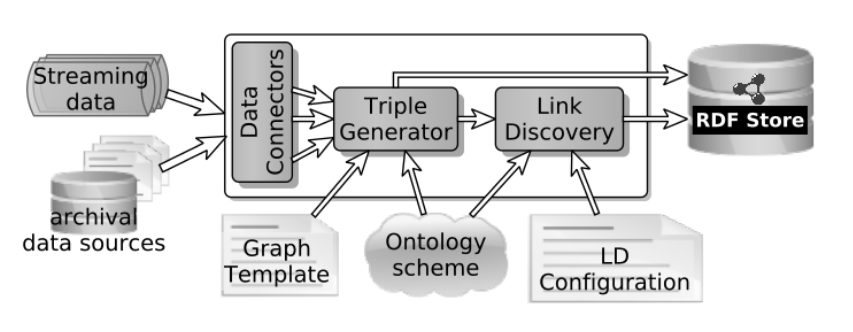
\includegraphics[width=0.8\textwidth]{fig/rdf-gen-arch.png}
  \caption{Architecture of RDF-Gen\cite{rdf_gen}}
  \label{fig:rdf-gen-arch}
\end{figure}

\subsubsection{Data Connector}
Data Connector has a similar functionality as the \emph{iterator functions} from SPARQL-Generate.
It consumes the data sources given a configuration setting. Configuration setting is used to specify 
the type of data sources, the \emph{window} for processing the incoming data records and 
also apply functions on the incoming data elements. Data Connector can thus be defined as a 
mapping function as in Definition~\ref{defn:data_connector}. 


\begin{defn}[Data Connector record \cite{rdf_gen}]
  \label{defn:data_connector}
  Given a set of data sources $D = \{d_1, d_2, \dots, d_n\}$ and  a 
  mapping function $F = \mu_{f}(d_i, e)\; |\; \forall d_i \in D$ with $e$, a data element 
  of a data source $d_i$, and $f$, a filter function. Data Connector 
  generates a record $R = \mu_{f}(d_i, e)$ $\iff$ all the attributes of 
  $e$ satisfy the filter function $f$. By default, the filter function $f$ just returns true. 
\end{defn}

Using the Definition~\ref{defn:data_connector}, we could now also apply an equi-join operator 
on the data sources. Formally, we could generate a new triple 
$R =  \mu_{f_i}(d_i, e_i) \bowtie  \mu_{f_j}(d_j, e_j) $ where $e_i$ and $e_j$ have 
common attributes under the filter functions $f_i$ and $f_j$. 

The processing is done on individual records, leading to 
RDF-Gen treating streaming and archival data sources the same way --- as “streams” 
of records. Due to the record-by-record processing, the framework also has a very low 
memory usage. 

\subsubsection{Triple Generator}
As indicated in Figure~\ref{fig:rdf-gen-arch}, Triple Generator consumes the output records 
of the Data Connectors to convert them into RDF triples. A vector of variables $V$, an RDF 
graph template $G$, akin to the basic graph pattern from SPARQL 1.1, and a 
set of functions can be used to configure the Triple Generators. 

$V$ consists of variables which corresponds to the attributes of the
generated records from the Data Connector. These variables are referenced 
in the graph template $G$, and then used to 
bind to the attribute value of the record provided by the Data Connector. Therefore, 
this simple binding of values in a template graph enables Triple Generator to 
generate RDF triples efficiently and have a high scalability.

Listing~\ref{lst:rdf_gen_example} shows an example graph template $G$ provided to 
the Triple Generator to generate RDF triples. In this example, the provided vector 
of variable is $V = [\textrm{?diagnosis\_id}, \textrm{?name} ]$.
\begin{lstlisting}[language={SPARQL},
   caption={A simple graph template $G$ with the functions \emph{asString} and \emph{makeUri}.}, 
   label={lst:rdf_gen_example}
  ]
  #BGP for the diagnosis data source
  makeUri(?diagnosis_id) a example:Diagnosis;
  example:name asString(?name).
\end{lstlisting}



\section{Mapping based Engines}

\subsection{RMLStreamer}
